\chapter{Metodología}

En el desarrollo de proyecto, al ser el desarrollo de una aplicación de Software, sumado al corto tiempo asignado para la actividad, se implementará una metodología ágil de SCRUM, cuyo seguimiento y control se realizará a partir de la herramienta HacknPlan.

\section{Metodología Ágil}

Día a día, el Software se vuelve más complejo y el manejo de herramientas ha evolucionado, volviéndose más sencillas y productivas de manejar, por ello, se requiere de una metodología de desarrollo de Software que se adapte a estos cambios.
La metodología de desarrollo de Software es un conjunto de "mejores prácticas" que si no se lleva a cabo, resulta inútil\cite{carrizo2018metodo}. Los recursos humanos son considerados como el factor más importante del proyecto de Software.

La metodología ágil de desarrollo de Software se fundamenta en los 4 principios básicos de la figura \ref{manifiesto}, que permite al equipo priorizar el Software que funciona a la documentación, rezagarse del uso de un diagrama relacionales hasta el final del desarrollo y una respuesta a cambios más versátil que en una planificación estricta.
\\
\begin{figure}[t!]
	\centering
	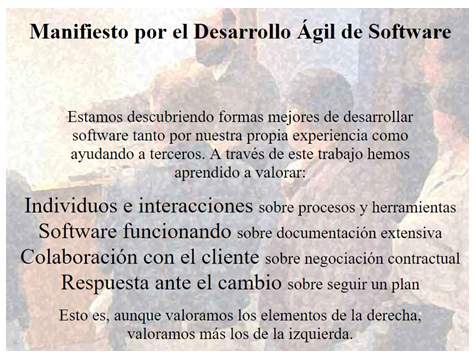
\includegraphics[width=13cm,height=5cm,]{./Images/manifiesto.png}
	\caption{Ejemplo de Clasificación de imagen de TensorFlow}
	\footnotesize Fuente: \cite{beck2001manifiesto}
	\label{manifiesto}
\end{figure}

De las metodologías ágiles conocidas, la más apropiada para el proyecto es la metodología SCRUM, debido a su seguimiento y comunicación, forzando a los miembros a un reporte diario y a un avance continuo con resultados productivos, con la posibilidad de definir metas en un tiempo específico, maximizando la efectividad de los recursos humanos.

\section{Metodología SCRUM}

La metodología SCRUM es una estrategia de gestión donde se aplica un conjunto de prácticas de manera regular para mejorar el trabajo colaborativo y obtener el mejor proyecto de Software posible\cite{scrumdiapo}.

Basado en la adaptabilidad, orientación a las personas y no los procesos y es iterativo e incremental. Requiere de la comunicación directa del cliente con el equipo desarrollador, el cual que será un miembro del equipo, al ser quien expuso, propuso y lideró el desarrollo.

La metodología SCRUM recibe los requisitos y los involucra como parte de la discusión de una reunión, para ser implementada. Se debe garantizar el desarrollo de los requisitos y permite detectar si estos producen conflictos.

\subsection{Componentes de SCRUM}

Para realizar el seguimiento de la metodología SCRUM, se requiere tomar nota de todas las decisiones realizadas, en general, la metodología fue seguida al pie de la letra, sin embargo, se destaca en Plan de Actividades, que hubo una pausa al avance del proyecto durante vasto tiempo, por tanto, se produjeron diversos cortes y extensiones de tiempo al momento de realizar las Sprint, posteriormente explicado en dicho subtitulo.

\subsubsection{Reuniones}

Las reuniones tienen el objetivo de definir cual es el trabajo que se debe realizar durante el Sprint.

\subsubsection{Project Backlog}
\subsubsection{Sprint Backlog}

\subsubsection{Roles de la Metodología SCRUM}

Se asigno a cada uno de los integrantes del equipo un rol distintivo y aparte el rol de SCRUM team.

\begin{itemize}
	\item \textbf{Product Owner:} Es la persona que conoce el panorama completo del producto y el entorno del negocio, representa a los usuarios del producto y es responsable del Product Backlog.
	\item \textbf{SCRUM Master:} Encargado de garantizar el funcionamiento de la metodología y evaluar los procesos, es una responsabilidad del funcionamiento del modelo, es un rol flexible del que depende el exito del proyecto.
	\item \textbf{Project Manager:} Es el encargado de dirigir el equipo a cumplir con los objetivos del equipo, se asegura de que los requerimientos se cumplan.
	\item \textbf{SCRUM Team:} Se le conoce asi a los integrantes del equipo de desarrollo, que produce resultados, cuyas habilidades son aptas para el desarrollo del proyecto de Software.
\end{itemize}




\subsubsection{Planning Poker}

\subsubsection{Herramienta GitHub}

\subsubsection{Reuniones Diarias}

\subsubsection{Horario de Trabajo}

\subsection{Sprints}

Un Sprint es también considerado una iteración y se realiza en la revisión de requisitos del usuario, el cual designa los requisitos del proyecto, traduciéndose tanto en tareas de usuario como en tareas para los desarrolladores, estas tareas se distribuyen en los distintos sprint.


\subsubsection{Sprint 1}

\subsubsection{Sprint 1}

\subsection{Gráfica Burn Up}

\subsection{Gráfica Burn Down}
